\setcounter{figure}{0}
\setcounter{table}{0}

\makeatletter
\renewcommand{\thefigure}{S\@arabic\c@figure}
\renewcommand{\thetable}{S\@arabic\c@figure}
\makeatother

\vfill

\begin{figure}[h]
\begin{align*}
  \frac{dT}{dt} &= R \cdot \alpha_T(T+M)[1-\alpha_B(B+M)] + M \cdot \theta\cdot \theta_T (1-\epsilon) - T \cdot \beta_B(B+M)(1-\epsilon) -T \cdot \epsilon \\
  \frac{dB}{dt} &= R \cdot  \alpha_B(B+M)[1-\alpha_T(T+M)] + M \cdot \theta (1- \theta_T) (1-\epsilon) - B \cdot  \beta_T(T+M)(1-\epsilon) -B \cdot \epsilon \\
  \frac{dR}{dt} &= \epsilon(M+B+T) - R \cdot \alpha_B(B+M)[1-\alpha_T(T+M)] - R \cdot \alpha_T(T+M)[1-\alpha_B(B+M)] - R \cdot \alpha_B(M + B) \alpha_T(M + T)\\
  \frac{dM}{dt} &=  B \cdot \beta_T(T+M)(1-\epsilon) +  T \cdot \beta_B(B+M)(1-\epsilon) + R \cdot \alpha_B(B+M)[1-\alpha_T(T+M)] - M \cdot \theta \cdot \theta_T (1-\epsilon) - M \cdot \theta (1- \theta_T) (1-\epsilon) - M \cdot  \epsilon\\
\end{align*}
\caption{All differential equations representing the boreal-temperate ecotone through four different states. B, M, R and T mean Boreal, Mixed, Regeneration and Temperate respectively.}
\label{EqSys}
\end{figure}

\vfill

\begin{table}[h]
	\begin{center}
		\caption{Transition and none-transition observed between two measurements through all plots surveys without regard to the time interval. B, M, R and T mean Boreal, Mixed, Regeneration and Temperate. }
		\label{TransMat}
		\begin{tabular}{c|cccc}
			 \diagbox{From}{To} &	\textbf{B} &     \textbf{M} &     \textbf{R} &     \textbf{T} \\
			\hline
			\textbf{B} & \textbf{15 357} &   794 &   203 &     - \\
			\textbf{M} &   302 & \textbf{14 433} &    51 &   959 \\
			\textbf{R} &   485 &    57 &   \textbf{209} &    80 \\
			\textbf{T} &     - &  891  &    40 & \textbf{15 134}
		\end{tabular}
	\end{center}
\end{table}

\vfill

\begin{figure}[h]
  \begin{center}
    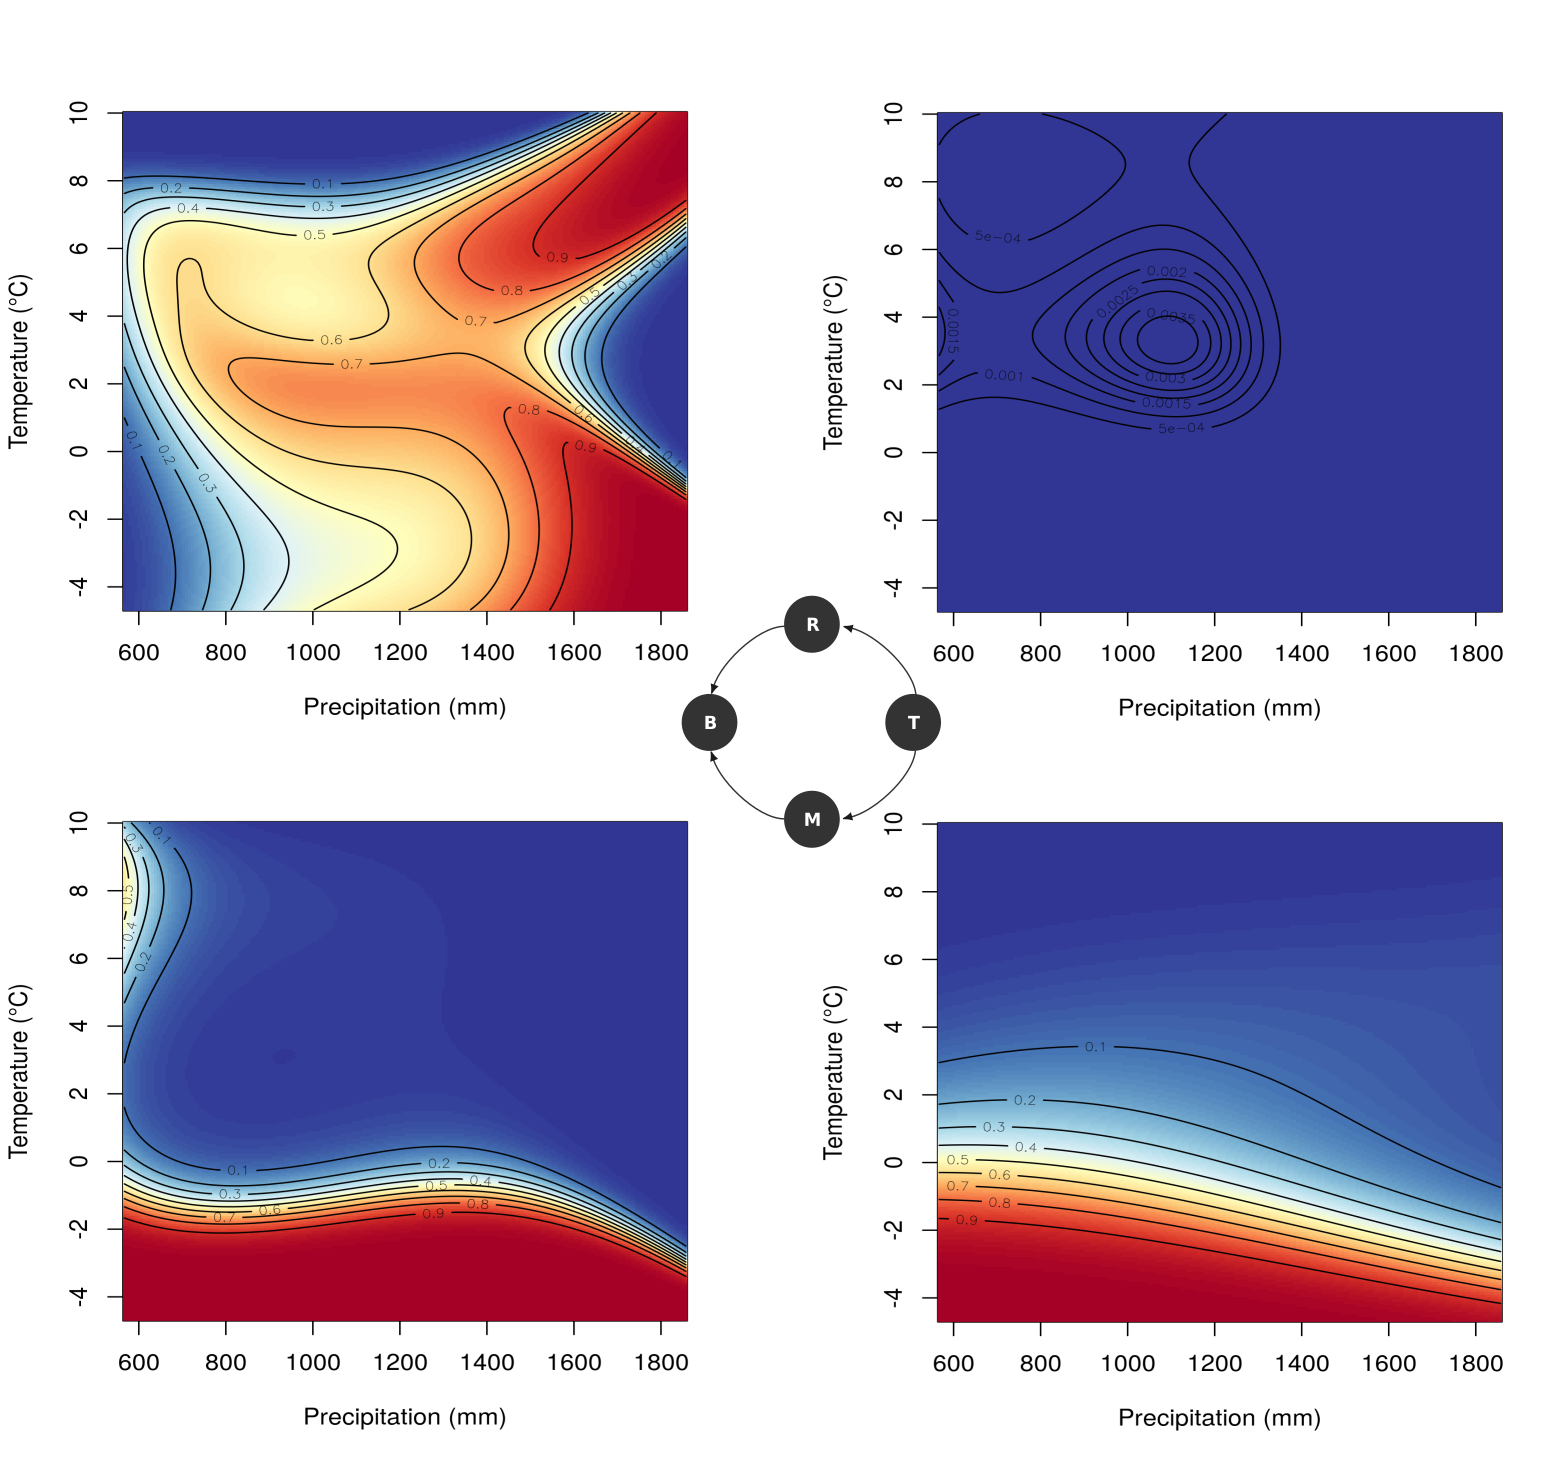
\includegraphics[width=\textwidth]{figs/trans_prob_SI.png}
    \caption{Illustration of the transition probabilities of all pathway driving the conversion of a state Temperate (T) to Boreal (B).  Probability functions are predicted by multinomial regression as a third degree polynomial which account for the temperature ($^{\circ}$Cs) and the precipitation (mm). Transition pathways are described by the arrows of the centered diagram.}
    \label{fig:SpaceSI}
  \end{center}
\end{figure}
\clearpage